% Options for packages loaded elsewhere
\PassOptionsToPackage{unicode}{hyperref}
\PassOptionsToPackage{hyphens}{url}
%
\documentclass[
]{book}
\usepackage{amsmath,amssymb}
\usepackage{lmodern}
\usepackage{iftex}
\ifPDFTeX
  \usepackage[T1]{fontenc}
  \usepackage[utf8]{inputenc}
  \usepackage{textcomp} % provide euro and other symbols
\else % if luatex or xetex
  \usepackage{unicode-math}
  \defaultfontfeatures{Scale=MatchLowercase}
  \defaultfontfeatures[\rmfamily]{Ligatures=TeX,Scale=1}
\fi
% Use upquote if available, for straight quotes in verbatim environments
\IfFileExists{upquote.sty}{\usepackage{upquote}}{}
\IfFileExists{microtype.sty}{% use microtype if available
  \usepackage[]{microtype}
  \UseMicrotypeSet[protrusion]{basicmath} % disable protrusion for tt fonts
}{}
\makeatletter
\@ifundefined{KOMAClassName}{% if non-KOMA class
  \IfFileExists{parskip.sty}{%
    \usepackage{parskip}
  }{% else
    \setlength{\parindent}{0pt}
    \setlength{\parskip}{6pt plus 2pt minus 1pt}}
}{% if KOMA class
  \KOMAoptions{parskip=half}}
\makeatother
\usepackage{xcolor}
\usepackage{longtable,booktabs,array}
\usepackage{calc} % for calculating minipage widths
% Correct order of tables after \paragraph or \subparagraph
\usepackage{etoolbox}
\makeatletter
\patchcmd\longtable{\par}{\if@noskipsec\mbox{}\fi\par}{}{}
\makeatother
% Allow footnotes in longtable head/foot
\IfFileExists{footnotehyper.sty}{\usepackage{footnotehyper}}{\usepackage{footnote}}
\makesavenoteenv{longtable}
\usepackage{graphicx}
\makeatletter
\def\maxwidth{\ifdim\Gin@nat@width>\linewidth\linewidth\else\Gin@nat@width\fi}
\def\maxheight{\ifdim\Gin@nat@height>\textheight\textheight\else\Gin@nat@height\fi}
\makeatother
% Scale images if necessary, so that they will not overflow the page
% margins by default, and it is still possible to overwrite the defaults
% using explicit options in \includegraphics[width, height, ...]{}
\setkeys{Gin}{width=\maxwidth,height=\maxheight,keepaspectratio}
% Set default figure placement to htbp
\makeatletter
\def\fps@figure{htbp}
\makeatother
\setlength{\emergencystretch}{3em} % prevent overfull lines
\providecommand{\tightlist}{%
  \setlength{\itemsep}{0pt}\setlength{\parskip}{0pt}}
\setcounter{secnumdepth}{5}
\usepackage{booktabs}
\ifLuaTeX
  \usepackage{selnolig}  % disable illegal ligatures
\fi
\usepackage[]{natbib}
\bibliographystyle{plainnat}
\IfFileExists{bookmark.sty}{\usepackage{bookmark}}{\usepackage{hyperref}}
\IfFileExists{xurl.sty}{\usepackage{xurl}}{} % add URL line breaks if available
\urlstyle{same} % disable monospaced font for URLs
\hypersetup{
  pdftitle={Buying Derivatives - A Monte Carlo Approach},
  pdfauthor={Jake Rozran},
  hidelinks,
  pdfcreator={LaTeX via pandoc}}

\title{Buying Derivatives - A Monte Carlo Approach}
\author{Jake Rozran}
\date{2023-04-18}

\begin{document}
\maketitle

{
\setcounter{tocdepth}{1}
\tableofcontents
}
\hypertarget{intro}{%
\chapter{Introduction}\label{intro}}

Over the past year, I've revolutionized the world of security\textsuperscript{\protect\hyperlink{def}{1}}
derivatives\textsuperscript{\protect\hyperlink{def}{2}} by developing an algorithm that calculates expected
outcomes with accuracy. Specifically, I've focused on the lucrative world of
put\textsuperscript{\protect\hyperlink{def}{3}} and call options\textsuperscript{\protect\hyperlink{def}{4}} on stocks - and I'm thrilled to share
my approach findings with you.

Using a cutting-edge Monte Carlo simulation\textsuperscript{\protect\hyperlink{def}{5}}, I've created a range of
probabilities\textsuperscript{\protect\hyperlink{def}{6}} that accurately reflect the expected gains and costs of
each option. By combining these probabilities, I've unlocked the secret to
calculating expected value\textsuperscript{\protect\hyperlink{def}{7}} with incredible accuracy - making it
easier than ever to decide which options to purchase and when.

In fact, I've already put my algorithm to the test with a variety of different
stocks - and the results are nothing short of astounding. With a winning
strategy in hand, you'll be able to confidently navigate the complex world of
security derivatives - and come out on top every time. So buckle up, and get
ready to join me on the forefront of financial innovation.

\hypertarget{mc}{%
\chapter{The Monte Carlo Engine}\label{mc}}

I am attempting to predict what the price of any stock will be at an options
expiration date, some days from now. The Monte Carlo simulation allows me to
create probabilities for different scenarios. To say that more precisely, the
simulation allows me to know the probability that an option will be in-the-money
on its expiration date.

As an example, I will predict what the price of Comcast (CMCSA) will be 30 days
from now.

The simulation is given all of the price change data from CMCSA back to 2000. It
calculates the daily price changes. The simulation then randomly picks from the
historical pot of price changes what the stock will do tomorrow and tomorrow and
tomorrow (and so on, up to the end date 30 days from now).

\begin{center}\includegraphics{_main_files/figure-latex/print_single-1} \end{center}

This gets you a single simulated possible path that the stock could take for the
next 30 days. It is unlikely - probably there is actually 0\% chance - that the
stock will actually follow that exact random path. Here's the magic of the
simulation: I then create 10,000 to 100,000 more random paths using the exact
same technique.

\begin{center}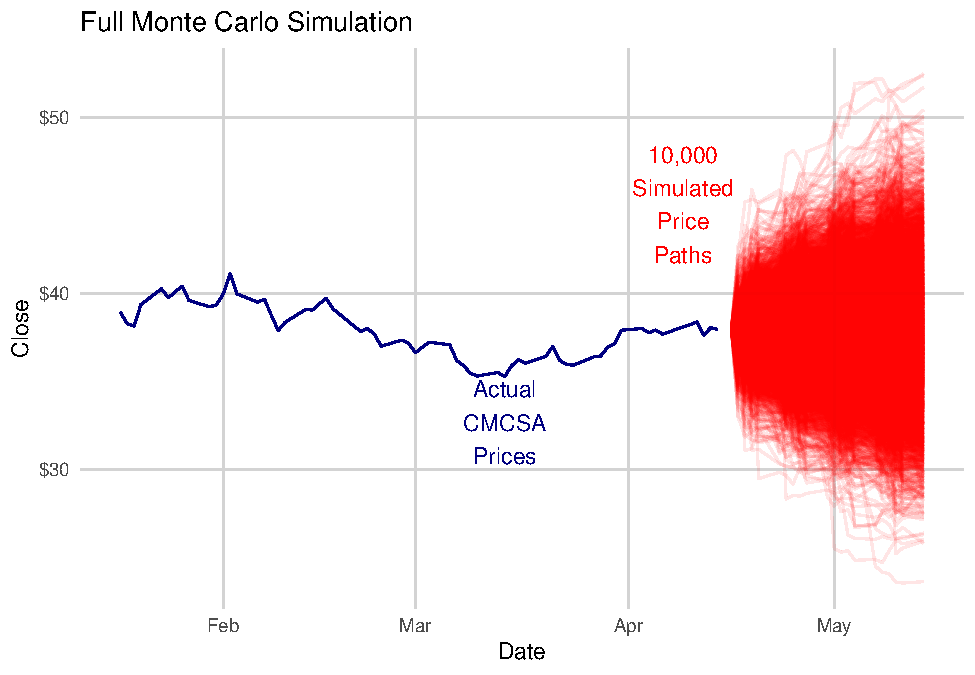
\includegraphics{_main_files/figure-latex/print_full-1} \end{center}

This full world of simulated price paths allows me to see the distribution of
potential prices at the option expiration date. I now know the average, median,
high, low, etc. price at the expiration date.

More beautifully, I can calculate probabilities that a stock price will reach
or exceed a strike price at a given options expiration date (more on that below).

\hypertarget{effective-price-and-being-in-the-money}{%
\section{Effective Price and Being In-The-Money}\label{effective-price-and-being-in-the-money}}

To find the probability that a certain option is in-the-money, we can simply
count the number of simulations that finish above (or below for a put) the
effective price (the strike plus the premium for the option) and divide by the
total simulations - this is the beauty of the monte carlo simulations.

\hypertarget{why-do-we-care-about-the-effective-price-instead-of-just-strike-price}{%
\subsection{Why do we care about the effective price (instead of just Strike Price)?}\label{why-do-we-care-about-the-effective-price-instead-of-just-strike-price}}

It is not enough to find out if an option will only go above its strike price.
You have to pay to own the option\ldots{} hence, you are already some money into the
deal. Since you've already paid some money, you need to make that money back,
too, to be in-the-money.

When the strike is in-the-money, the premium to buy the option will be large
enough to make the effective price equal to the current price. The more
in-the-money, the higher the premium.

When the strike is out-of-the-money, the premium will be smaller. The further
out-of-the-money a strike is, the lower the premium.

\hypertarget{lets-look-at-an-example.}{%
\subsection{Let's look at an example.}\label{lets-look-at-an-example.}}

CMCSA is currently trading at \$38.09. Let's use a call option
with a strike of \$42 that has a premium of \$0.05. The effective price of the
option (for a call) is: \$42 + \$0.05 = \$42.05.

What is the probability that we meet or exceed that effective price on the
strike date? To find that out, we count the number of all of the simulations
that ended with a price greater than or equal to the effective price and divide
that by the total count of simulations.

In this case, we have 964 simulations that are in-the-money
out of a total 10,000, or
9.64\% chance that this
option ends in the money.

\begin{center}\includegraphics{_main_files/figure-latex/print_histogram-1} \end{center}

\hypertarget{expected-stock-price-if-in-the-money}{%
\section{Expected Stock Price if In-The-Money}\label{expected-stock-price-if-in-the-money}}

Now that I know the probability of it going above the effective price, I need to
calculate the expected price of the stock if it is in-the-money. To do this, I
simply take all simulations that end at or above the effective price and
calculate the expected value (or mean).

\begin{center}\includegraphics{_main_files/figure-latex/print_ev-1} \end{center}

\hypertarget{bringing-it-all-together-expected-value-of-the-option}{%
\section{Bringing it all Together: Expected Value of the Option}\label{bringing-it-all-together-expected-value-of-the-option}}

I have the probability the option will end in-the-money (and by definition the
probability that the option will end out-of-the-money). I also know the premium
to buy the option and the expected price of the stock if it is above the
effective price. I am ready to calculate the expected value of the option.

\begin{itemize}
\tightlist
\item
  It costs \$5 to buy the option (100 shares at \$0.05 each)
\item
  There is a 9.64\% chance
  the option ends in-the-money
\item
  There is a 90.36\% chance the option ends
  out-of-the-money
\item
  If the option ends in the money, the stock is expected to be at
  \$43.89, which is equivalent to a gain of \$43.89 -
  \$42.05, or \$1.84 (times 100 shares)

  \begin{itemize}
  \tightlist
  \item
    The gain if the option ends in the money is \$183.58
  \item
    The final gain, minus the \$5 to buy the option in the first place, is
    \$178.58
  \end{itemize}
\item
  Putting all of that together, buying this option is worth
  \textbf{\$12.70}

  \begin{itemize}
  \tightlist
  \item
    There is a 10\% chance you make \$178.58
  \item
    There is also a 90\% chance you just lose your \$5 premium
  \item
    This expected value is really only possible if you execute this plan
    many many independent times over the long run
  \end{itemize}
\end{itemize}

\hypertarget{evaluating-the-portfolio}{%
\chapter{Evaluating the Portfolio}\label{evaluating-the-portfolio}}

THIS IS WHERE I SHOW HOW TO PICK OPTIONS

One thing to consider is the correlation between the stocks.

\hypertarget{the-business-plan}{%
\chapter{The Business Plan}\label{the-business-plan}}

What if I had \$10MM? How would I use it?

Part of the money goes to making recurring bets on options - that's where the
big break comes from. I can't put all my eggs in that basket, though\ldots{} that's
dumb. So to round things out, part of the unused cash should go into short
term investments: a mixture of high yield savings accounts, money market
accounts, and CDs. I can also stash some cash in stock index funds and bond
index funds.

\hypertarget{appendix-appendix}{%
\appendix}


\hypertarget{def}{%
\chapter{Definitions}\label{def}}

\begin{enumerate}
\def\labelenumi{\arabic{enumi}.}
\item
  In finance, a security refers to a tradable financial asset that has monetary
  value and can be bought or sold in a financial market. Securities include a wide
  range of assets, such as stocks, bonds, options, futures, and exchange-traded
  funds (ETFs), among others.\protect\hyperlink{intro}{↩︎}
\item
  A derivative is a financial instrument whose value is derived from the value
  of an underlying security, such as a stock, bond, commodity, or currency.
  In other words, the value of a derivative depends on the value of the underlying
  asset. There are many types of derivatives, including options, futures,
  forwards, and swaps.For example, an option is a type of derivative that
  gives the holder the right, but not the obligation, to buy or sell an underlying
  asset at a specific price within a specified time period.\protect\hyperlink{intro}{↩︎}
\item
  A put option is a type of financial contract that gives the holder the right,
  but not the obligation, to sell an underlying security at a predetermined price
  (known as the strike price) within a specific period of time (known as the
  strike date).In other words, a put option gives the holder the ability
  to sell an asset at a certain price, even if the market price of the asset falls
  below the strike price. This can be useful for investors who believe that the
  price of an asset is likely to decline, as it allows them to profit from the
  decline without actually owning the asset.For example, if an investor
  buys a put option for a certain stock with a strike price of \$50 and an
  expiration date of one month, and the stock's market price falls to \$40 during
  that time, the investor can exercise the put option to sell the stock at the
  higher strike price of \$50, making a profit of \$10 per share. However, if the
  stock's market price remains above the strike price of \$50, the investor may
  choose not to exercise the put option and will lose the premium paid to purchase
  the option.\protect\hyperlink{intro}{↩︎}
\item
  A call option is a type of financial contract that gives the holder the
  right, but not the obligation, to buy an underlying asset, such as a stock,
  bond, or commodity, at a predetermined price (known as the strike price) within
  a specific period of time.In other words, a call option gives the holder
  the ability to purchase an asset at a certain price, even if the market price of
  the asset rises above the strike price. This can be useful for investors who
  believe that the price of an asset is likely to increase, as it allows them to
  profit from the increase without actually owning the asset.For example,
  if an investor buys a call option for a certain stock with a strike price of
  \$50 and an expiration date of one month, and the stock's market price rises to
  \$60 during that time, the investor can exercise the call option to buy the
  stock at the lower strike price of \$50, making a profit of \$10 per share.
  However, if the stock's market price remains below the strike price of \$50,
  the investor may choose not to exercise the call option and will lose the
  premium paid to purchase the option.\protect\hyperlink{intro}{↩︎}
\item
  A Monte Carlo simulation is a computational method used to estimate the
  probability distribution of an outcome by generating a large number of random
  samples or scenarios and analyzing their aggregate behavior.\protect\hyperlink{intro}{↩︎}
\item
  Probability is a measure of the likelihood or chance that a specific event
  will occur, expressed as a number between 0 and 1.A probability of 0
  means that the event is impossible, while a probability of 1 means that the
  event is certain to occur. A probability of 0.5 (or 50\%) means that the event
  has an equal chance of occurring or not occurring.\protect\hyperlink{intro}{↩︎}
\item
  Expected value is a concept used in statistics to calculate the long-term
  average value of a random variable, taking into account the probability of each
  possible outcome.The expected value is calculated by multiplying each
  possible outcome by its probability and adding up all the products. In other
  words, it is the weighted average of all possible outcomes.\protect\hyperlink{intro}{↩︎}
\end{enumerate}

\hypertarget{calculating-an-options-expected-value}{%
\chapter{Calculating an Option's Expected Value}\label{calculating-an-options-expected-value}}

The expected value for each option can be calculated as follows:

\begin{equation} 
E_p(k) = (P_{ae} * C) + (P_{be} * G)
\label{eq:puts}
\end{equation}

\begin{equation} 
E_c(k) = (P_{be} * C) + (P_{ae} * G)
\label{eq:calls}
\end{equation}

where

\begin{itemize}
\tightlist
\item
  \(E_p(k)\) is the expected value of a put at strike price \(k\)
\item
  \(E_c(k)\) is the expected value of a call at strike price \(k\)
\item
  \(P_{ae}\) is the probability a security price on the strike date is above the
  \emph{effective price}\footnote{The effective price is the strike price plus the option cost
    (for calls) - you cannot make money on the option until you cross this
    threshold}, \(k_e\)

  \begin{itemize}
  \tightlist
  \item
    This is calculated with the Monte Carlo simulation
  \item
    \(P_{ae} = \frac{r_{ae}}{r_t}\) where \(r_{ae}\) is the number of runs above
    the expected price and \(r_t\) are the total runs
  \end{itemize}
\item
  \(P_{be}\) = 1 - \(P_{ae}\) is the probability a security price on the strike date
  is below the \emph{effective price}, \(k_e\)
\item
  \(C = 100c\) is the cost to buy the option

  \begin{itemize}
  \tightlist
  \item
    \(c\) is the cost of a single option (options are typically bought/sold in
    lots of 100)
  \end{itemize}
\item
  \(G = 100(E_{p_s}(p_s|p_s>k_e) - c)\) is the expected gain if the derivative
  is in the money

  \begin{itemize}
  \tightlist
  \item
    \(E_{p_s}(p_s|p_s>k_e)\) is the expected value of the of the price of the
    stock, \(p_s\), given that the price of the stock has exceeded the effective
    price, \(k_e\) (for calls).
  \end{itemize}
\end{itemize}

\end{document}
